\chapter{Fundamentação teórica e metodologia}

\section{\dBG}

The \dBG is a very nice structure to represent sets of related kmers.... One example of such a beautiful structure is shown in Figure~\ref{fig:dbgexample}.

\begin{figure}[htbp]
	\begin{center}
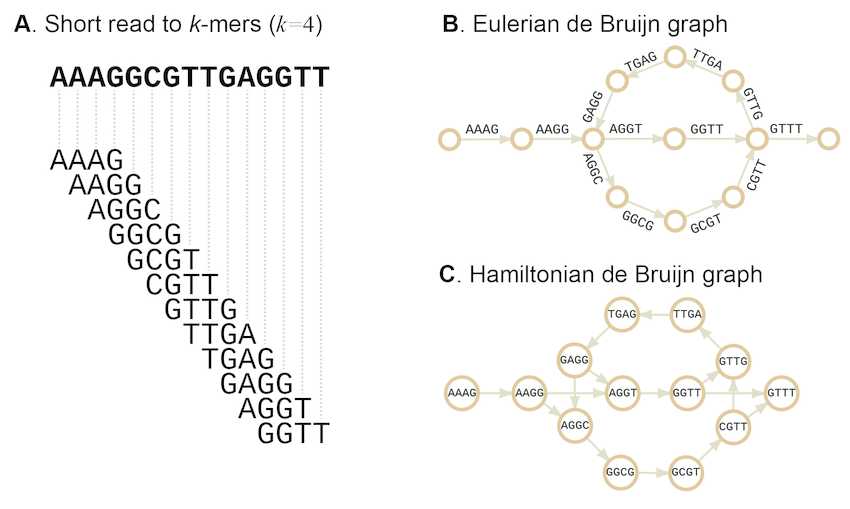
\includegraphics[width=10cm]{dbg}
$$E=mc^2$$
	\end{center}
	\caption{Example of a \dBG.}\label{fig:dbgexample}
\end{figure}


- Detailed explanation of \dBG of a set of DNA sequences
  - reverse complements
- How it is going to be used
- Operations
  - Insert node
  - Insert edge
  - Query node
  - Query edge / star 
- Space-efficient representations - that's what we propose

\section{Outline of construction/representation}

Sequence ---(insert)---> Mod CountMin ---(traverse)---> Hashtable 


\section{CountMin sketch}

\section{Modified CountMin sketch}

- Representation (what goes in each cell)
- Operations:
  - addOutEdge
  - query 
- Analysis space/time (may be done within previous sections)

The \emph{de~Bruijn} CountMin sketch is defined very similarly to the original CountMin sketch, the only difference being that instead of only storing counters in each cell, the set of out edges are also stored.
This set is restricted, due to the nature of a \emph{de~Bruijn} graph, to the edges represented by the four bases $\{\A, \C, \G, \T\}$.
In order to store this additional information, we must define a new operation on the CountMin sketch, the \textbf{addOutEdge(k-mer, outEdge)} operation.
This new operation adds the given out edge to the set of out edges of the given key in all corresponding cells. The query operation must also be updated
to account for the new information that must be retrieved and must return a set of out edges along with the estimated count for the given key.
The logic for obtaining the estimate for the count remains the same, and is paralleled in the process of obtaining the set of out edges to be returned.
An out edge is said to exist for the given key if and only if it is found in all of the cells corresponding to that key. I.e. the set of out edges
returned by the query operation is the intersection of all the sets of out edges associated with the given key. This behavior is also similar to that
implemented in Bloom Filters.

In order to implement this in a space-efficient manner, both out edges and counter are stored in a single 16 bit integer. The first 4 bits
function as flags to indicate the presence of the out edges, with $b_1 = A, b_2 = C$, etc. The remaining 12 bits are the actual counter.
In this way, the \textbf{increment(k-mer)} operation can be implemented as usual, by simply incrementing the value of each cell associated with the key,
while the \textbf{addOutEdge(k-mer, outEdge)} can be done by setting the bit corresponding to the given out edge to one in all those same cells.
The \textbf{query(\kmer)} operation can retrieve the count associated with the given key by using a bit-mask for the 12 least significant bits of each
cell and then taking the minimum value as usual, while the out edges can be obtained by performing a bitwise AND between 4 most significant bits
in each cell.

It should be noted that, due to the context of sequencing reads, counts are only ever \emph{incremented} and out edges are only ever \emph{added},
such that an \textbf{incrementBy(k-mer, count)} operation, a \textbf{decrement(k-mer)} operation or a \textbf{removeOutEdge(k-mer, outEdge)} operation will never be needed and,
therefore, are not defined.

\paragraph{Presence.} A k-mer is considered to be present in the graph if and only if the estimated count returned by the query operation
is above a certain threshold. This threshold should be defined as a function of the expected count for a real k-mer (i.e. the sequencing coverage).

\paragraph{Adding out edges.} An out-edge is recorded to a k-mer by taking the last base of it's following k-mer. This update is only done,
however, once the latter is found to be present in the graph. In this way, we avoid storing spurious out edges for erroneous k-mers.
iiThis presence requirement is only applied to the head k-mer.

\begin{algorithm}[htbp]
    \caption{$\mathit{addOutEdge}(\text{k-mer}, \mathit{outEdge})$}\label{alg:addOutEdge}
    \begin{algorithmic}
        \Ensure $\mathit{outEdge} \in \{A, C, G, T\}$
        \For{$i = 1, \ldots, D$}
            \State $\mathit{CountMin}[i][h_i(\text{k-mer})].\mathit{outEdges} \gets \mathit{CountMin}[i][h_i(\text{k-mer})].\mathit{outEdges} \cup \mathit{outEdge}$
        \EndFor
    \end{algorithmic}
\end{algorithm}

\begin{algorithm}
    \caption{$\mathit{query}(\text{k-mer})$}\label{alg:query}
    \begin{algorithmic}
        \State $\mathit{count} \gets \mathit{inf}$
        \State $\mathit{outEdges} \gets \{A, C, G, T\}$
        \For{$i = 1, \ldots, D$}
            \State $\mathit{count} \gets \min(\mathit{count}, \mathit{CountMin}[i][h_i(\text{k-mer})].\mathit{count})$
            \State $\mathit{outEdges} \gets \mathit{outEdges} \cap \mathit{CountMin}[i][h_i(\text{k-mer})].\mathit{outEdges}$
        \EndFor
    \end{algorithmic}
\end{algorithm}


\section{Hashtable}
- Structure
  - fingerprint
  - Outedges
- Hash function 
- Collision resolution
- Operations 
  - Add node/edge
  - Query node/edge/star 
- Analysis 





